\section{am::lambda::binder2$<$ R, P1, P2, A1, A2 $>$ Struct Template Reference}
\label{structam_1_1lambda_1_1binder2}\index{am::lambda::binder2@{am::lambda::binder2}}
{\tt \#include $<$lambda.hpp$>$}

Inherits {\bf am::lambda::detail::lambda\_\-op\_\-tag}.

Inheritance diagram for am::lambda::binder2$<$ R, P1, P2, A1, A2 $>$:\begin{figure}[H]
\begin{center}
\leavevmode
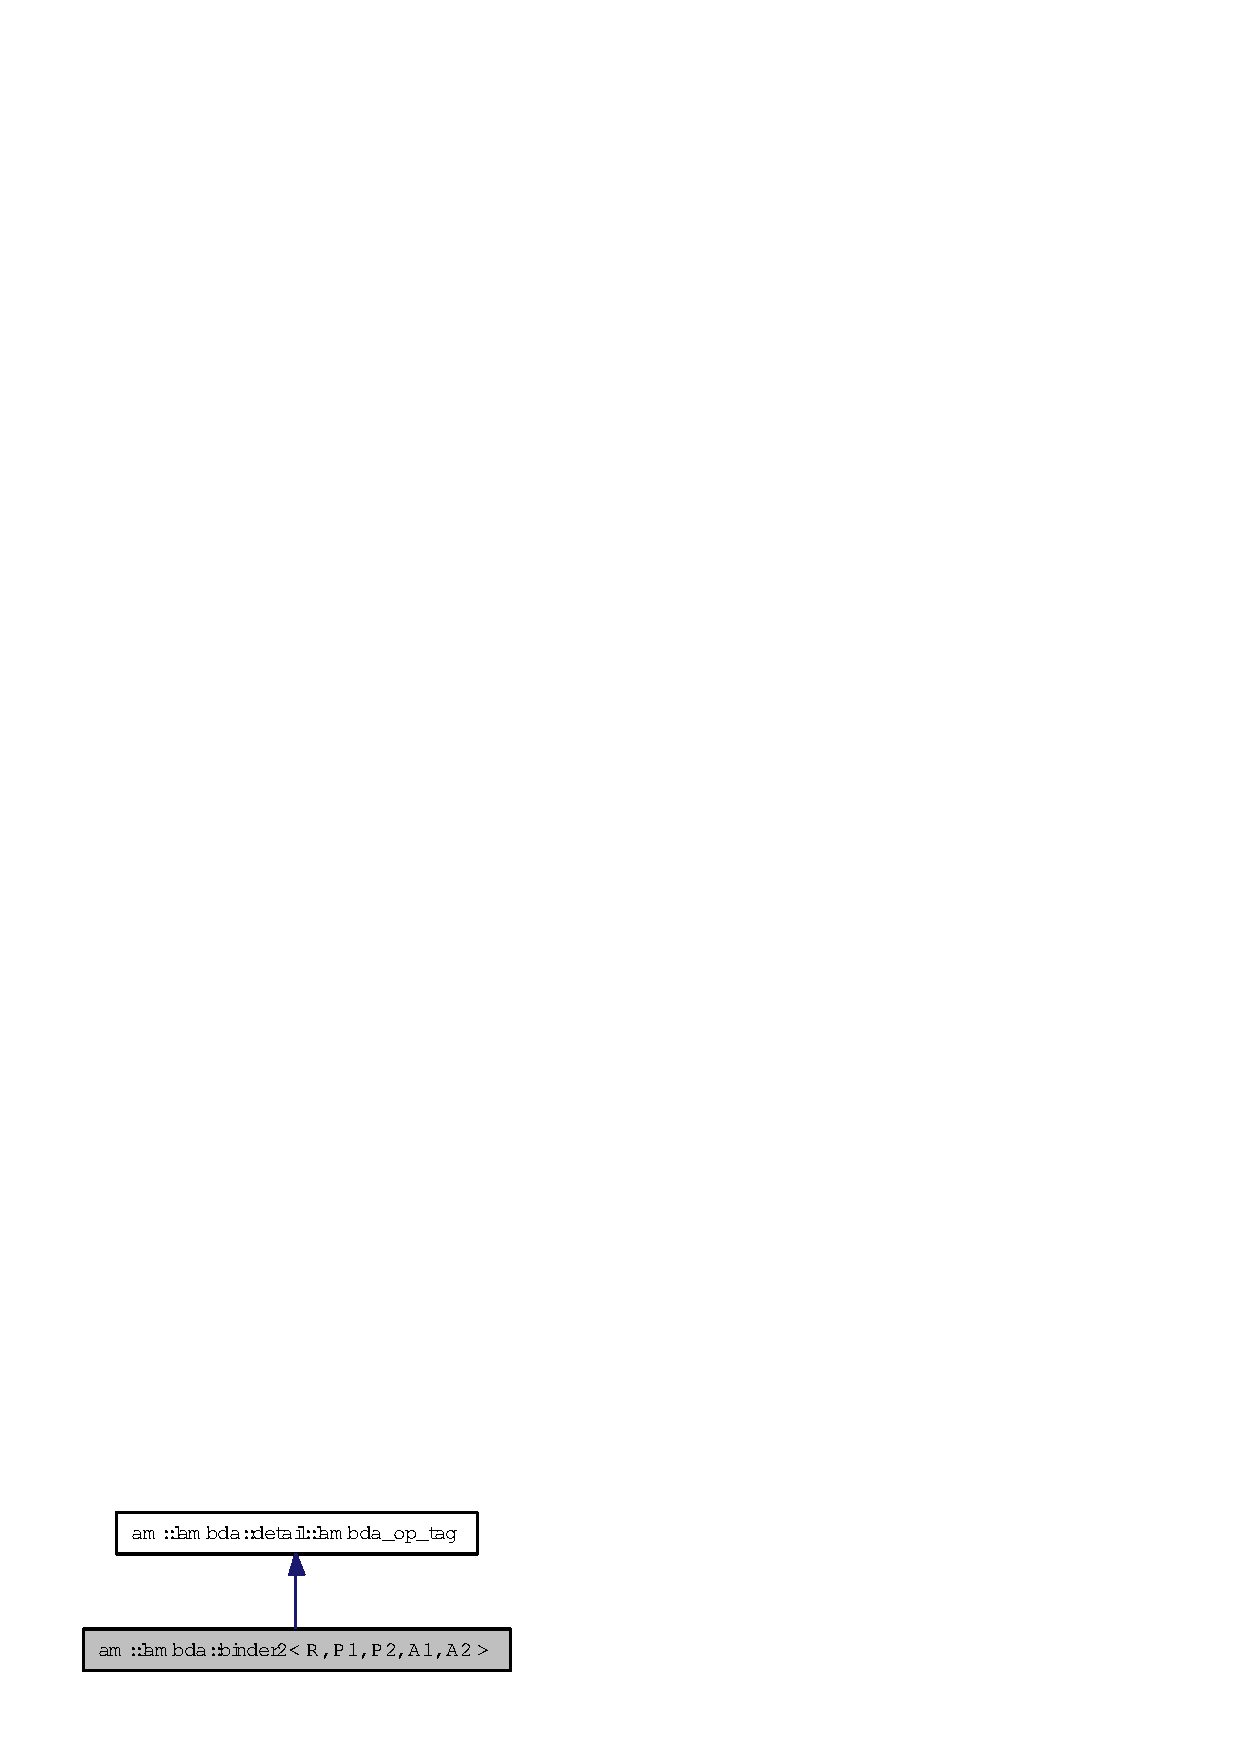
\includegraphics[width=124pt]{structam_1_1lambda_1_1binder2__inherit__graph}
\end{center}
\end{figure}
Collaboration diagram for am::lambda::binder2$<$ R, P1, P2, A1, A2 $>$:\begin{figure}[H]
\begin{center}
\leavevmode
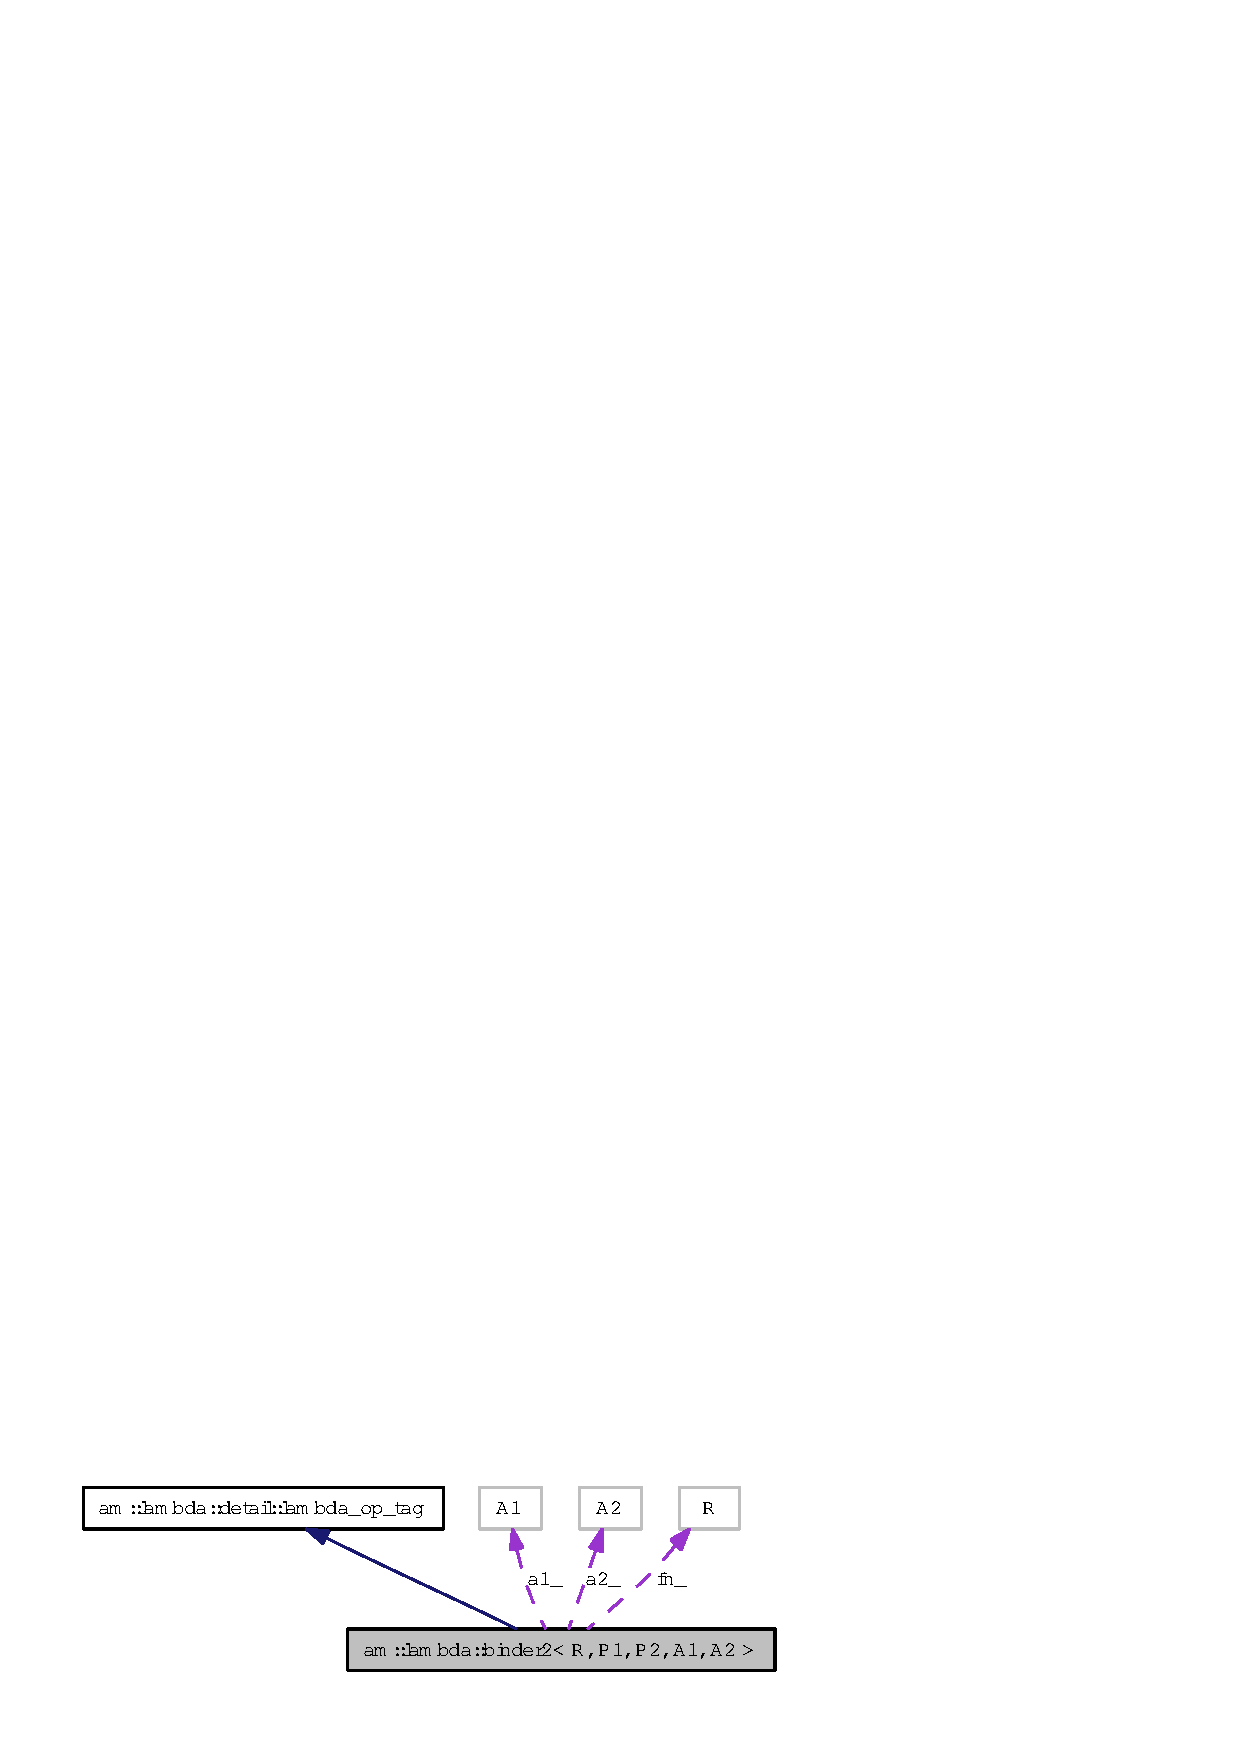
\includegraphics[width=187pt]{structam_1_1lambda_1_1binder2__coll__graph}
\end{center}
\end{figure}
\subsection*{Public Types}
\begin{CompactItemize}
\item 
typedef detail::binder\_\-impl$<$ R $>$::result\_\-type \textbf{result\_\-type}\label{structam_1_1lambda_1_1binder2_d73405ab552afa44c840d27cd4709304}

\end{CompactItemize}
\subsection*{Public Member Functions}
\begin{CompactItemize}
\item 
\textbf{binder2} (R($\ast$fn)(P1, P2), A1 a1, A2 a2)\label{structam_1_1lambda_1_1binder2_4d517a5e99db7eb10225d490c802fa74}

\item 
template$<$class T1, class T2, class T3$>$ result\_\-type \textbf{operator()} (T1 t1, T2 t2, T3 t3) const \label{structam_1_1lambda_1_1binder2_8c204abc6133be2e95cd176639f52448}

\item 
template$<$class T1, class T2$>$ result\_\-type \textbf{operator()} (T1 t1, T2 t2) const\label{structam_1_1lambda_1_1binder2_2019db2e2568b959a5e5f5ad3b77f900}

\item 
template$<$class T1$>$ result\_\-type \textbf{operator()} (T1 t1) const \label{structam_1_1lambda_1_1binder2_3576ec06cf7e48b3b7346eeeecbb20dc}

\item 
result\_\-type \textbf{operator()} () const\label{structam_1_1lambda_1_1binder2_08f8cf7c190fc6e5e46e13010a9a86f9}

\end{CompactItemize}
\subsection*{Public Attributes}
\begin{CompactItemize}
\item 
R($\ast$ \textbf{fn\_\-} )(P1, P2)\label{structam_1_1lambda_1_1binder2_b214a0c003ee4e9c8ac97fda0bca30a9}

\item 
A1 \textbf{a1\_\-}\label{structam_1_1lambda_1_1binder2_ce8184c78e50af5a002839aba6b1351a}

\item 
A2 \textbf{a2\_\-}\label{structam_1_1lambda_1_1binder2_0de68b465afbb45b7304a96a1f6d671a}

\end{CompactItemize}


\subsection{Detailed Description}
\subsubsection*{template$<$typename R, typename P1, typename P2, typename A1, typename A2$>$ struct am::lambda::binder2$<$ R, P1, P2, A1, A2 $>$}

Binder for the free function which takes two arguments. 



The documentation for this struct was generated from the following file:\begin{CompactItemize}
\item 
{\bf lambda.hpp}\end{CompactItemize}
